\documentclass{article}
\usepackage{fancyhdr,booktabs}
\usepackage{amsmath}
\usepackage{float}
\usepackage{graphicx}
\usepackage{indentfirst}
\usepackage{geometry}
\usepackage{citesort}

\begin{document}

\section{Numerical Methods}
\cite{kludge}
\section{Confusion problem}

Given a waveform under spacetime with non-zero deformation parameter, in order to see if there is "confusion problem", we need to decide which waveform under Kerr spacetime is most similar to it and look at their overlap. Here we search for existence confusion problem with similar method as \cite{majorPRD}.

If we restrict ourselves to equatorial motion, set the initial $t$ and $\phi$ to 0 taking advantage of symmetry and set initial $r=r_{max}$ imposing the phase to match, then orbital eccentricity $e$, semilatus rectum $p$, BH mass $M$ and BH spin $a$ are the parameters that determine the motion.

According to Ref. \cite{sameOmg}, orbits with same orbital frequency $\omega_r$ and $\omega_\phi$ can generate most similar gravitational waveforms. Here we check this result by looking at overlaps between waveform of ($\delta_1,\, a,\, M,\, e,\, p$) = (0.2, 0.5, $2 \times 10^5 $ , 0.5, 6) and of ($\delta_1,\, a,\, M,\, e,\, p$) = (0, 0.5, $2 \times 10^5 $ , $e_{Kerr}$, $p_{Kerr}$). First we look at overlap distribution on a relatively large range of (e, p). Then we search near ($e_{Kerr}$, $p_{Kerr}$) with same orbital frequency, as shown in Fig. \ref{overlapdist}. 

Note that the difference between equating $\omega^{(t)}$, orbital frequency with respect to coordinate time, and $\omega^{(\tau)}$, orbital frequency with respect to proper time, can be significant. From Fig. \ref{overlapdist} it is explicit that the same orbital frequency with respect to t can result in almost the largest overlap while the same orbital frequency with respect to $\tau$ cannot. In Kerr spacetime, the expression for $\omega^{(t)}$ and $\omega^{(\tau)}$ are given in \cite{tOmg} and \cite{tauOmg}.

\begin{figure}[]
	\centering
	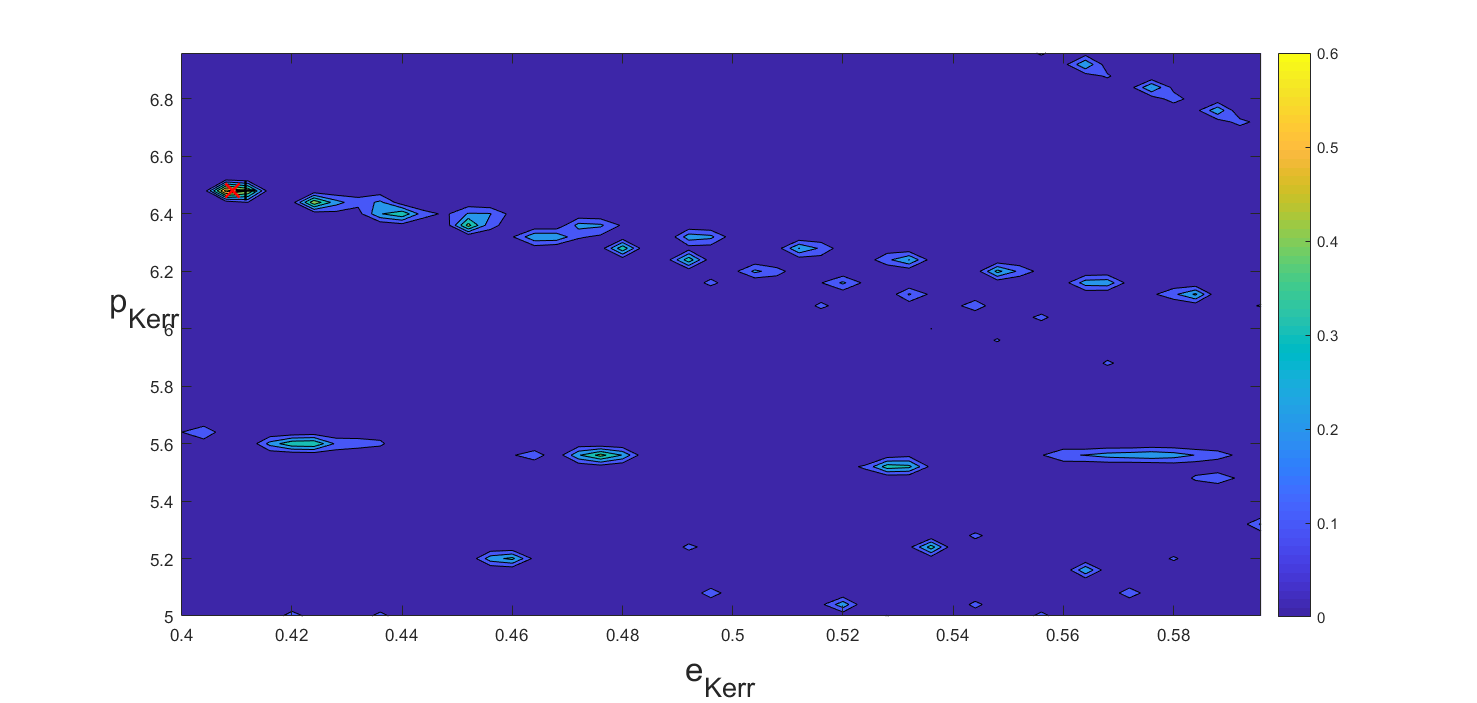
\includegraphics[width=16cm]{OLdist.png}
	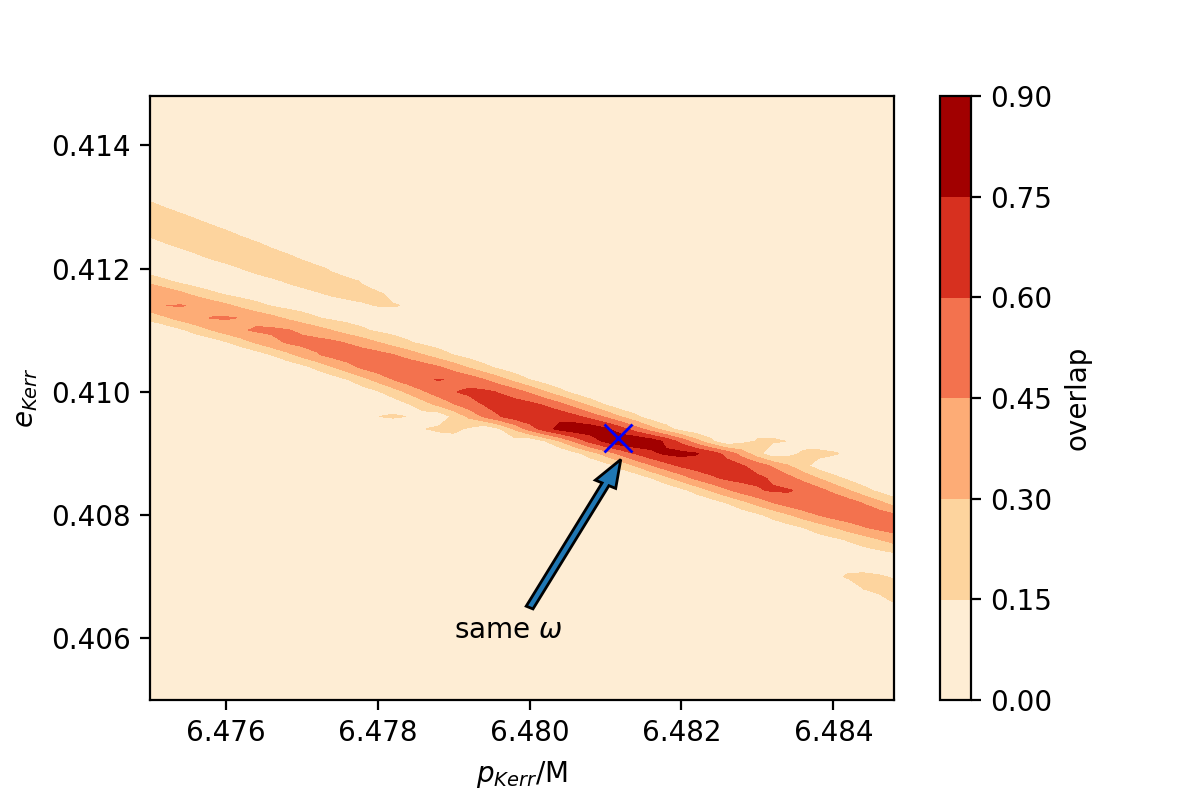
\includegraphics[width=16cm]{OLdist2.png}
	
	\caption{Distribution of overlap between waveform of ($\delta_1,\, a,\, M,\, e,\, p$) = (0.2, 0.5, $2 \times 10^5 $, 0.5, 6) and waveforms of ($\delta_1,\, a,\, M,\, e,\, p$) =(0, 0.5, $2 \times 10^5 $, $e_{Kerr}$, $p_{Kerr}$) on ($e_{Kerr}$, $p_{Kerr}$) plane. The original data are both 50*50 grid. Red cross mark: same $\omega^{(t)}$ at ($e_{Kerr}$, $p_{Kerr}$) = (0.409248, 6.481170), overlap is 0.8912. Black plus mark: same $\omega^{(\tau)}$ at  ($e_{Kerr}$, $p_{Kerr}$) = (0.411495, 6.482549), overlap is 0.0507 }
	\label{overlapdist}
\end{figure}

This result is explicit by looking at the waveforms over a relatively long time (here about $50000M$), as shown in Fig. \ref{kkwave}. 

\begin{figure}[!htb]
	\centering
	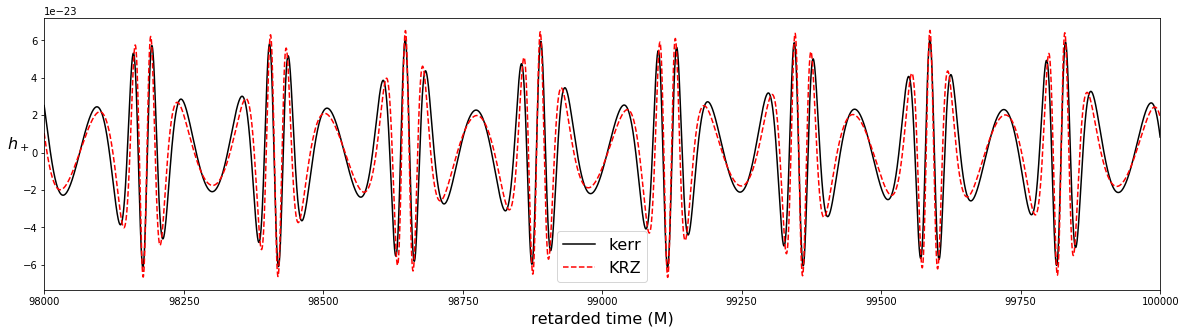
\includegraphics[width=16cm]{krz_kerr_wave.png}
	
	\caption{Comparison between waveforms of $h_+$ with respect to retarded time in units of central black hole mass $M$. The black solid line is the waveform under $\delta_1=0.2$, e=0.5,p=6. The red dashed line is the waveform under $\delta_1=0$ and e, p adapted so that the orbital frequencies with respect to t $\omega^{(t)}_r$ and $\omega^{(t)}_\phi$ are the same as that of the orbit under d1=0.2, e=0.5, p=6. The green dotted line is the waveform under $\delta_1 =0$ and e, p adopted so that $\omega^{(\tau)}$s are the same . The spin of the central black hole is 0.5M.}
	\label{kkwave}
\end{figure}	
	
Therefore we regard waveforms in Kerr spacetime with same orbital frequencies with respect to proper time as best matches to waveforms in non-Kerr space time under KRZ parametrization.

Fig. shows the overlap distribution...

As Fig. suggest, the confusion problem still exists in KRZ parametrization. The deformation parameter $\delta_1$ is kind of degenerated with   in Kerr spacetime. This resulted can also be found by looking at covariance matrix as discussed in next section
\section{Constraints on deformation parameter by future LISA task}

\bibliography{citation}
\bibliographystyle{plain}
\end{document}